%
% Szakdolgozatminta az Eszterházy Károly Katolikus Egyetem
% matematika illetve informatika szakos hallgatóinak.
%

\documentclass[
% opciók nélkül: egyoldalas nyomtatás, elektronikus verzió
% twoside,     % kétoldalas nyomtatás
% tocnopagenum,% oldalszámozás a tartalomjegyzék után kezdődik
]{thesis-ekf}
\usepackage[T1]{fontenc}
\usepackage{hyperref}
\usepackage{graphicx}
\PassOptionsToPackage{defaults=hu-min}{magyar.ldf}
\usepackage[magyar]{babel}
\usepackage{mathtools,amssymb,amsthm,pdfpages}
\footnotestyle{rule=fourth}

\newtheorem{tetel}{Tétel}[chapter]
\theoremstyle{definition}
\newtheorem{definicio}[tetel]{Definíció}
\theoremstyle{remark}
\newtheorem{megjegyzes}[tetel]{Megjegyzés}

\begin{document}

\institute{Matematikai és Informatikai Intézet}
\title{A szakdolgozat címe}
\author{Bartus János\\Programtervező informatikus}
\supervisor{Troll Ede\\Tanársegéd}
\city{Eger}
\date{2025}
\maketitle

\tableofcontents

\chapter*{Bevezetés}
\addcontentsline{toc}{chapter}{Bevezetés}
Gyerekkorom óta érdekeltek a videójátékok, már egészen kicsiként kezdtem el játszani. Az első komolyabb élményeimet apukám PlayStation 2 konzolján szereztem ahol sok időt töltöttem különböző játékokkal. Akkoriban még csak a játék öröme vonzott, nem is gondoltam volna hogy ennyire mélyen elmerülök ebben a világban.
Ahogy idősebb lettem, általános iskola alsó tagozatában kezdtek jobban érdekelni a videójátékok nemcsak mint szórakozás hanem mint rendszerek. Elkezdtem azon gondolkodni hogyan működnek, mi és hogy irányítja a karaktereket és a játékon belüli eseményeket.
 
A programozás irányába a Minecraft vezetett. Felfedeztem benne a parancsblokkokkat és azokkal próbáltam változtatni a játék világát. Egyre izgalmasabbá vált hogy a saját ötleteimet meg tudom valósítani, ekkor határoztam el hogy programozó akarok lenni.

A programozással középiskolában kezdtem el komolyabban foglalkozni. Ekkor már tudatosan kerestem azokat a lehetőségeket, amelyekkel jobban megérthetem hogyan működnek különböző játékok és szoftverek. Az első lépéseimet kisebb programok megírásával kezdtem. Kezdetben iskolai beadandók során próbáltam ki magam, de rájöttem hogy a játékfejlesztés felé saját projektekkel lehet jobban elmélyedni. Ezért elkezdtem kisebb játékokat és interaktív szoftvereket fejleszteni, amivel nemcsak a programozás alapjait tudtam gyakorolni, hanem a játékok logikáját is elkezdtem jobban megérteni.

Komolyabban foglalkozni a programozással egyetem alatt kezdtem el. Ebben az időszakban rengeteg új dolgot tanultam, és megismerkedtem számos különböző programozási nyelvvel és technikával. Az egyetem nemcsak az elméleti tudást adta meg, hanem lehetőséget adott, hogy gyakorlati tapasztalatot szerezzek különböző feladatok és projektek révén.

A számomra eddig ismeretlen platformer játék stílussal is az egyetem alatt ismerkedtem meg. Az első találkozásom ezzel a műfajjal izgalmas kihívások elé állított amely lehetőséget adott arra, hogy új területeken is kipróbáljam magam a játékfejlesztésben. A platformerek különlegessége számomra az volt, hogy egyesíteni kell bennük a szórakoztató játékmechanikát, a kreatív pályadizájnt és az erőteljes történetmesélést. Az igazi áttörés az egyetem megrendezésre kerülő GémDzsem alatt tapasztam. Olyan hatással volt rám ez az élmény hogy eldöntöttem: szeretnék a játékfejlesztéssel komolyan foglalkozni.

A szakdolgozatom során először készítek platformer játékot, amelynek animációit és grafikáit  egy grafikus tervezi és készíti el. Ez új kihívást jelent számomra, mivel a játékmenet mellett most a vizuális elemekre is nagyobb figyelmet kell fordítanom, és együtt kell működnöm egy más emberrel, hogy a játék mind vizuálisan, mind technikailag sikeres legyen. Az együtt működés lehetőséget ad arra hogy jobban megismerjem vizuális elemek kezelését, mivel eddig nem sokat dolgoztam grafikákkal.

Forráskód elérhetősége: \href{https://github.com/bartusjani/W5OLP9_szakdolgozat}{github.com/bartusjani/W5OLP9\_szakdolgozat}

Játék elérhetősége: \href{https://example.com}{example.com}

Bemutató videó elérhetősége: \href{https://example.com}{example.com}


\chapter{Technológiai áttekintés}

\section{Godot Engine}

A Godot Engine egy nyílt forráskódú és ingyenes . Általános célú 2D és 3D játékmotor, ami mindenféle projektet támogat. Lehetővé teszi a játékok kiadását különböző platformokra. A Godotban lehet C\#,C++ vagy GDScripttel programozni.
\subsection{GDScript nyelv}
A GDScript Godot specifikus nyelv. Ez a programozási nyelv egy objektumorientált, imperatív, magas szintű nyelv. A Pythonhoz hasonló behúzásalapú szintaxist használ. A Godot Enginehez optimalizált és integrált, célja hogy nagy rugalmasságot biztosítson a szoftverfejlesztéshez. A GDScript a Pythontól  teljesen független, és nem arra épül.

A GDScript azonosítói kizárólag betűket (a-z, A-Z), számokat (0-9) és aláhúzás jelet tartalmazhatnak. Fontos hogy az azonosító nem kezdődhet számjeggyel.A nyelv kis és nagybetű érzékeny tehát például valtozo és a VALTOZO mást különböző változónak számítanak. Támogatja a  UAX\#31 szabványú Unicode karaktereket.

Az egész és lebegőpontos számokat aláhúzással (\_) elválasztva is lehet írni. Például 123456789-et lehet 123\_456\_789-nek írni és a nyelv fel fogja ismerni.

A kommentet a Pythonhoz hasonlóan \#-el lehet tenni. Lehet a kommentekből régiót csinálni ami össze csukható.A régiót így lehet csinálni \#region ... \#endregion.

\subsubsection*{Beépített adattípusok}
Alapértelmezés szerint veremalapú objektumokként tárolódnak, amely érték szerint kerülnek átadásra.

\textbf{Alapvető beépített típusok:}
\begin{itemize}
	\item null
	\item bool
	\item int
	\item float
	\item String
	\item StringName \\ Egy nem módosítható karakterlánc, ami biztosítja, hogy egy adott szöveg csak egyszer legyen a memóriában. Bár létrehozása erőforrás-igényesebb, gyorsabb összehasonlítást tesz lehetővé, ezért ideális szótárkulcsokhoz.
	\item NodePath \\ Egy előfeldolgozott útvonal csomópontokhoz, amely könnyen átalakítható String típusúvá. 
\end{itemize}
\textbf{Vektor adattípusok:}
\begin{itemize}
	\item Vektor2, Vektor2i \\ 2D vektor típus ami x és y mezőt tartalmaz. A Vector2i-nél csak integer lehet az x és y mezőben.
	\item Vector3, Vector3i \\ 3D vektor típus ahol x és y mező mellett van y mező is. Itt is csak integer lehet a Vector3i mezőiben.
	\item Transform2D \\ Egy 3×2-es mátrix, ami 2D transzformációk végrehajtására alkalmas. 
	\item Transform3D \\ Egy 3D transzformációt reprezentáló típus, amely egy Basis mezőből és egy Vector3 mezőből áll.
	\item Basis \\ Egy 3x3-as mátrix amit 3D forgatás és skálázásra használnak.
\end{itemize}

\subsection{A Godot verzóinak áttekintése}
A Godot Engine-t folyamatosan fejlesztik , rendszeresen új funkciókkal, teljesítménybeli javításokkal és hibajavításokkal frissül.Az alábbiakban a legfontosabb verziókról fogok írni.
\begin{itemize}
	\item[$\bullet$] Godot 1.0 \\ 2014 decemberében jelent meg a Godot Engine első stabil verziója. Több száz hibát javítottak és a közösség is jelentősen megnövekedett.
	\item[$\bullet$] Godot 2.0 \\ 2016 februárjában jelent meg.A Godot 2.0-ban javították jelenetpéldányosítást.Bevezették a jelenet öröklést és egy új szöveges jelenetformátumot ami könnyeben kezelhető, Git kompatibilis és gyorsabb. Továbbá támogatja az onready kulcsszót és singeltonokat.
	\item[$\bullet$] Godot 3.0 \\ 2018 januárjában jelent meg. A Godot 3.0-ban új fizikai alapú 3D renderelő kapott helyet. Behozták a GDNative-ot  ami egy új keretrendszer amivel könnyen bővíthető a Godot C/C++ nyelven a motor újrafordítás nélkül.
	\item [$\bullet$] Godot 4.0\\  2023 márciusában jelent meg és jelentős javításokat hozott .  A Godot 4.0-ban a 2D munkafolyamatokban új tilemap szerkesztőt vezettek be amivel könnyebb a szint tervezés. A 3D területén a shader-ek és VFX rendszerek újításokon estek át, emellett jelentős fejlesztéseket kapott és shader szerkesztő is.
\end{itemize}
Most a legfrissebb verziója a Godot 4.4.1 amit 2025 márciusában adtak ki.
\subsection{Licenszi kérdések}
A Godot az MIT licenc alatt készült és kerül kiterjesztésre. Az MIT licenc egyetlen követelménye, hogy a licenc szövegét valahol a játékban el kell helyezni.
\subsection{A motor fő erősségei}
\begin{itemize}
	\item Intuitív jelenetvezérelt tervezés \\ A játékokat egyszerű blokkokból építheted fel, ahol a csomópontok (nodes) hierarchiája segít az átlátható kialakításában.
	\item Testre szabott kódolási eszközök \\ A GDScript és C\# nyelvek biztosítanak gyors fejlesztést, míg a Godot 4.0 új statikus típusellenőrzése növeli a hatékonyságot és teljesítményt.
	\item Egyszerű, mégis nagy teljesítményű 3D motor \\ Támogatja a magas és az alacsony teljesítményű eszközöket, a Vulkan renderelő kiaknázza a játék GPU-k erejét.
	\item Speciális 2D munkafolyamat játékokhoz és alkalmazásokhoz \\ A dedikált 2D tile map editor lehetővé teszi a gyors világépítést, egyszerűsíti a logikát és a GUI rendszert a játékokhoz.
\end{itemize}
\section{Unreal Engine}

Az Unreal Engine az Epic Games által fejlesztett, nagy teljesítményű játékmotor.Az első verzióját 1998-ban adták ki. A legfrissebb verziója az Unreal Engine 5. A motor támogatja a C++ programozási nyelven való fejlesztést, de a Blueprint rendszere lehetővé teszi a vizuális programozást is. A motor teljesen ingyen használható egy bevételi határ alatt, így lehetőséget ad a kisebb fejlesztők számára is.

\subsection{Blueprint}
A Blueprint a játékmotor egyik fontos eszköze, amely lehetővé teszi a játékok,alkalmazások logikájának vizuális szkriptelését. Különösen hasznos a nem programozó felhasználóknak, mivel így mélyebb programozási tudás nélkül is képesek a projektjeiket megvalósítani.
\subsubsection{A vizuális programozás erősségei}
A Blueprint egy teljes játékmenet--szkriptrendszer, amely csomópont--alapú koncepción alapul. Objektumorientált osztályok vagy objektumok definiálására szolgál a motorban.Ez a rendszer rendkívül rugalmas és nagy teljesítményű,lehetővé teszi a tervezők számára, hogy az általában csak a programozók számára elérhető fogalmak és eszközök teljes skáláját használhassák.

Számos előnyt kínál a fejlesztés során. Lehetővé teszi az egyszerűbb definiálását a viselkedéseknek, ami megkönnyíti a szkriptelést és a projekt logikájának kialakítását. Ideális eszköz a prototípusok készítésére, mivel gyorsítja az osztályok létrehozását,módosítását,lefordítását és tesztelését ezzel jelentős időt spórol meg.Az API-k gyorsabb felfedezését is lehetővé teszi.
\subsubsection{Blueprint osztályok}
A Blueprint osztály egy olyan eszköz, ami lehetővé teszi a új funkciók hozzáadását a játékmenethez kód írása nélkül.Eszközökként mentődnek el a tartalom csomagban.
\begin{itemize}
	\item[$\bullet$] Data--Only Blueprint \\ Ez egy olyan osztály ami csak örökölt kódot, változókat, komponenseket tartalmaz. Lehetővé teszi ezek változtatását, de új elemeket nem lehet hozzáadni. Archetípusok helyettesítésére szolgál. Teljes Blueprintté alakítható ha kódot, változókat vagy komponenseket adunk hozzá.
	\item[$\bullet$] Level Blueprint \\ A Level Blueprint egy speciális Blueprint típus, amely a teljes szint globális eseménygrafikájaként működik. Ez a Blueprint eseményeket, műveleteket kezel szintben lévő szereplőkkel kapcsolatban.
	\item[$\bullet$] Blueprint Utilities \\ A Blueprint Utility csak a szerkesztőre korlátozódik.Lehetővé teszi a szerkesztőben különböző  műveletek végrehajtását vagy funkciók hozzáadását a szerkesztőben. Gyakran használják szkriptek, szerkesztőbeli kiegészítők létrehozására. 
\end{itemize}

\subsection{Unreal Engine verzióinak áttekintése}
A Unreal Engine-t folyamatosan fejlesztik , rendszeresen új funkciókkal, teljesítménybeli javításokkal és hibajavításokkal frissül.Az alábbiakban pár újabb verzióról fogok írni.
\begin{itemize}
	\item[$\bullet$]Unreal Engine 4.27 \\ 2021 augusztusában jelent meg. Ez a verzió mindenki számára kínál valamit kezdve a filmesektől, vizualizációs szakembereken át a játékfejlesztőkig. Ebben a kiadásban a munkafolyamatok egyszerűsítésén és a teljesítmény növelésén volt a hangsúly.
	\item[$\bullet$]Unreal Engine 5.0 \\ 2022 áprilisában jelent meg. Ezen kiadásban a lehetővé tették a fejlesztők számára hogy next-gen valós idejű 3D tartalmakat,élményeket hozzanak létre nagyobb szabadsággal,rugalmassággal és részletességgel.Az új funkciók mint a Nanite vagy a Lumen új vizuális minőséget biztosítanak, lehetővé téve a dinamikus világok létrehozását.
	\item[$\bullet$]Unreal Engine 5.3 \\ 2023 szeptemberében jelent meg. Ez a kiadás tovább javította a UE5 eszközöket.Fejlesztették a renderelést, világépítést, procedurális tartalomgenerálást,animációs és modellezési eszközöket, a szimulációkat. Ezáltal az Unreal Engine 5.3 kiadás tovább erősítette az Epic Games elkötelezettségét a valós idejű grafika és fejlesztői eszközök élvonalbeli fejlesztése iránt.
	\item[$\bullet$]Unreal Engine 5.5 \\ 2024 novemberében jelent meg. Ez legfrissebb verziója az Unreal Engine-nek. Jelentős előrelépések történtek az animációk készítésében, a virtuális produkcióban és a mobiljáték--fejlesztésben területén is.Több funkció (például az in--camera--VFX, fejlesztői iteráció) elérte a gyártáskészséget. 
\end{itemize}
\subsection{Licenszi kérdések}
Az Unreal Engine-t az Egpic Games licencfeltételei alapján használható.Alapvetően ingyenesen elérhető, viszont egy meghatározott bevételi küszöb felett a fejlesztő köteles fizetni a játékmotor használatáért.Az alábbi felsorolásban ismertetem a különböző licenc lehetőségeket.
\begin{itemize}
	\item[$\bullet$] 1 millió dollár alatti bevétel esetén \\ Ingyenes a játék fejlesztők, egyéni fejlesztők, kisebb cégek,valamint iskolák és oktatók számára.
	\item[$\bullet$]1 millió dollár feletti bevétel esetén \\  Kétféle fizetési lehetőség közül választhat a fejlesztő:
	\begin{itemize}
		\item jogdíj alapú fizetés \\Ha olyan játékot vagy alkalmazást készít a fejlesztő, amely futásidőben használja az Unreal Engine kódját, és harmadik fél számára kerül licencelésre, akkor kell jogdíjat fizetnie.
		
		Költség: Az 1 millió dollárt meghaladó bevétel után 5\% jogdíjat kell fizetni.
		\item Ülőhely alapú fizetés \\ Ha az Unreal Engine-t kereskedelmi célokra használja a fejlesztő,és az elmúlt 12 hónapban több mint 1 millió dollár bevételt termelt,és nem olyan játékot vagy alkalmazást készít, amely futásidőben használja az engine kódját és harmadik félnek licencelhető, akkor ülőhely(seat) licenc díjat kell fizetnie.
		Költség: Évi 777 549 Ft / ülőhely.
	\end{itemize}
\end{itemize}
\subsection{A motor fő erősségei}
Az Unreal Engine számos erősséggel rendelkezik, amelyek hozzájárulnak ahhoz, hogy az egyik legnépszerűbb játékmotor legyen a piacon. Íme néhány főbb erőssége:
\begin{itemize}
	\item[$\bullet$] Grafikai teljesítmény \\Kiváló vizuális minőséget kínál, beleértve a valós idejű ray tracinget, amely valósághű fény- és árnyékhatásokat biztosít.
	\item[$\bullet$] Blueprint rendszer \\ A vizuális szkriptnyelv lehetővé teszi, hogy kódolás nélkül fejlesszünk játékokat, így gyors prototípusokat készíthetünk.
	\item[$\bullet$] Platform támogatás \\Az Unreal Engine támogatja a legtöbb nagy platformot, beleértve a PC-t, konzolokat, mobil eszközöket és VR/AR eszközöket. Ez lehetővé teszi a fejlesztők számára, hogy széles körű közönséghez juttassák el alkotásaikat.
\end{itemize}


\section{Unity}
A Unity egy rendkívül népszerű és széles körben használt játékmotor. A Unityben lehetőség nyílik játékok, interaktív élmények és egyéb 3D- és 2D-alapú alkalmazások fejlesztésére.A fejlesztők különböző platformokon (például PC, konzolok, mobiltelefonok, VR/AR eszközök) készíthetnek a Unityvel alkalmazásokat.
\subsection{Programozási nyelv}
A Unityben a programozás alapértelmezetten  C\#--ban történik.A C\# egy objektum--orientált programozási nyelv,amelyet a Microsoft fejleszt, és népszerű nyelv mivel könnyen tanulható és erőteljes eszközt biztosít a komplex játékmechanikák létrehozásához.
\subsubsection{C\# Főbb jellemzői}
\begin{itemize}
	\item[$\bullet$]Objektum--orientált \\Lehetővé teszi a kódok szervezését osztályok és objektumok formájában, megkönnyítve ezzel a karbantartást és a bővítést.
	\item[$\bullet$]Garbage collection\\A C\# automatikusan kezeli a memóriát egy beépített szemétgyűjtő rendszer segítségével, ami csökkenti a memóriaszivárgás és a memória kezelése körüli hibák kockázatát.
	\item[$\bullet$]Kivételkezelés\\A C\# támogatja a kivételkezelést.Try--catch blokkokat alkalmaz, amely lehetővé teszi a hibák hatékony kezelését és a program hibamentes futását.
	\item[$\bullet$]Kompatibilitás a .NET és Mono környezetekkel\\A C\# kódot futtathatjuk a .NET keretrendszeren és az open-source Mono környezeten is, így lehetővé téve az alkalmazások futtatását különböző platformokon mint például Windows,Linux és macOS.
\end{itemize}
\subsection{fontosabb verziók}
A Unity folyamatosan fejlődő és frissülő játékmotor, amelyet az Unity Technologies fejlesztett ki.Az alábbiakban pár verziójáról fogok írni.
\begin{itemize}
	\item[$\bullet$]Unity 4.0\\2012 novemberében jelent meg. A Unity 4.0--nak a célja a meglévő technológia javítása és új funkciók bevezetése volt. Főbb újítások:
	\begin{itemize}
		\item Fejlett vizuális képességek minden platformra\\Mobil platformokon is real-time árnyékok, skinned mesh instancing, normál térképek használata a fényképekhez.
		\item Mecanim animációs rendszer \\ Fejlett karakteranimációk létrehozására, beleértve az állapotgépeket, blend tree-ket, és auto retargetinget különböző karakterekhez.
		\item DirectX 11 támogatás \\ Teljes támogatás a shader model 5, tesszeláció és compute shaderek használatára a jobb grafikai teljesítmény érdekében.
	\end{itemize}
	\item[$\bullet$]Unity 5.0\\2015 márciusában jelent meg. Jelentős grafikai fejlesztésekkel és bővített szerkesztői funkciókkal jelent meg. Az új verzió lehetővé teszi a fejlesztők számára, hogy gyönyörű és innovatív játékokat készítsenek 21 platformra.
	\item[$\bullet$]Unity 6\\2024 októberében jelent meg. Jelenleg ez a legfrissebb verziója a Unitynek. A verzió számos fejlesztést és újítást tartalmaz, ezek közül párat részletesebben is leírok:
	\begin{itemize}
		\item Grafikai teljesítmény javítás \\A GPU Resident Drawer lehetővé teszi, hogy nagyobb és részletesebb világokat rendereljünk hatékonyan, miközben csökkenti a CPU költségeket. A GPU Occlusion Culling segítségével csak azokat az objektumokat rendereljük, amelyek láthatóak a képernyőn, így optimalizálva a teljesítményt. Ezen kívül a Render Graph technológia, amely különösen mobilplatformokon hasznos, javítja a memória- és energiahatékonyságot, míg a PC-k és konzolok esetében magasabb szintű testre szabhatóságot biztosít.
		\item Több játékos fejlesztések \\A  Unity 6 erősíti a multiplayer fejlesztést a Multiplayer Center-el, amely egy központi hubként szolgál, segítve a multiplayer eszközök és szolgáltatások kiválasztását, anélkül, hogy bonyolult technológiai döntéseket kellene hozni.
		\item Több platformos fejlesztés \\A Unity 6 egy új munkafolyamatot vezet be a Build Profile és Platform Browser funkciókkal, amelyek segítenek jobban kezelni és testreszabni a különböző platformokra készült build-eket.
		\item Ai és vizuális fejlesztések \\Az Adaptive Probe Volumes (APV) automatikusan elhelyezi a fénypróbákat, így gyorsabbá téve a fényalapú közvetett világításokkal való munkát.Az új Sentis AI lehetővé teszi a testreszabott AI modellek gyors integrálását.
	\end{itemize}
\end{itemize}
\subsection{licenszelési kérdések}
A Unity licencelési rendszer különböző típusú felhasználók és fejlesztők számára biztosít hozzáférést a motor különböző funkcióihoz. Az alábbi felsorolásban írok egyes licencekről.
\begin{itemize}
	\item[$\bullet$] Unity Student \\ Ingyenes. kizárólág diákok vehetik igénybe.
	\item[$\bullet$] Unity Personal\\ Ingyenes. Bárki használhatja.
	\item[$\bullet$] Unity Pro\\200\$ /hónap. Ezzel lehet konzolokra is kiadni.
	\item[$\bullet$] Unity Enterprise\\A legnagyobb vállalatok számára kínált lehetőség. Ez a verzió a legfejlettebb eszközöket és prémium támogatást biztosít, és általában személyre szabott megoldásokat kínál.
\end{itemize}
\subsection{főbb erősségei}
A Unity számos erősséggel rendelkezik, ebből párat részletesebben leírok.
\begin{itemize}
	\item[$\bullet$]Egyszerűsített multiplayer játékfejlesztés \\  A Unity 6 integrált multiplayer platformot kínál, amely gyorsítja a játékok online funkcióinak fejlesztését és tesztelését, megkönnyítve a többjátékos élmények létrehozását. 
	\item[$\bullet$]Fejlettebb mesterséges intelligencia képességek \\Az új Sentis eszközkészlet lehetővé teszi a fejlesztők számára, hogy AI modelleket integráljanak a játékokba, dinamikus és interaktív élményeket teremtve ezzel a játékosok számára. 
	\item[$\bullet$]Ray Tracing támogatás \\  Unity 6 natív támogatást ad a Ray Tracing API-hoz, lehetővé téve a fejlettebb és realisztikusabb fény-- és árnyékolási effektusok alkalmazását,amik a grafikai minőséget jelentősen megemelik.
\end{itemize}
Ezek a fejlesztések a Unity 6-ban jelentősen növelik a játékfejlesztés hatékonyságát és minőségét, kielégítve a modern fejlesztők igényeit.


\subsection{Jelenetek}
A Unity-ben a fejlesztés jelenetekben (scenes) történik, amelyek a játék vagy alkalmazás különböző részeit reprezentálják. Minden jelenet önálló egységként működik, és különféle GameObjecteket, komponenseket, valamint beállításokat tartalmazhat, amelyek együtt alkotják az adott rész működését és megjelenését.
\subsection{GameObject}
Unityben a GameObject reprezentál mindent ami egy jeleneten belül lehet. A GameObject osztály sok metódussal rendelkezik amivel segíti a programozást, például GameObjectek közötti keresés,üzenetküldés, a GameObjectekhez kapcsolt komponensek hozzáadása vagy eltávolítása.

\subsubsection{Komponensek}
A komponensek minden GameObjectnek funkcionális darabjai.A komponensek szerkesztésével lehet a GameObjectek viselkedését módosítani.Komponenst lehet hozzáadni,szerkeszteni vagy törölni a GameObjectről .Egy GameObjectnek lehet több komponense is, viszont egy Transform komponenssel muszáj rendelkeznie, mivel ezzel lehet a GameObjectnek meghatározni a helyét, forgatását és a méretarányát.

Ebben a szekcióban bemutatom részletesebben azokat a komponenseket amiket használtam a szakdolgozatom megírása során.

\subsubsection{Transform}
A Transform  mint fentebb említettem a GameObject helyét, forgatását és méretarányát tárolja a jelenetben.A 2D térben a Transzformokat csak az x- vagy az y-tengelyen lehet módosítani.A 3D térben x-,y- és z-tengelyen lehet módosítani.  A Unityben ezeket a tengelyeket a piros, a zöld és a kék színek jelölik.Ezeket lehet módosítani a jelenetben, a kódban vagy az inspector ablakban.
\subsubsection{Collider}
A Collider a Unity egyik legfontosabb alap komponense, amely lehetővé teszi hogy a GameObjectek fizikai kölcsönhatásba lépjenek egymással.A Collider egy fizikai határvonalat (ütköződobozt) határoz meg egy GameObject körül. Ez a határvonal láthatatlan a játékban, de a fizikai motor (Rigidbody) használja az ütközések, érintkezések, áthaladások stb. kezelésére.Collidert lehet 2D vagy 3D játékfejlesztésben is használni. A Collidereknek van isTrigger opciójuk ami ha be van állítva akkor nem ütköznek össze másik colliderekkel, de eseményeket tud kiváltani.Sok különböző alakú Collider létezik például néhány fajtája:
\begin{itemize}
	\item Circle Collider 2D/3D
	\item Box Collider 2D/3D
	\item Capsule Collider 2D/3D
\end{itemize}

\subsubsection{RigidBody}
A RigidBody2D lehetővé teszi a fizikán alapuló viselkedést, például a gravitációt, tömeget lehet vele módosítani.Ez mozgatja a GameObjectet felülírva a Transform komponenst.RigidBody komponenst lehet használni 2D vagy 3D játékfejlesztésben is. Ha Collider komponens is van a GameObjecten akkor együtt mozog a RigidBody--val.

\subsubsection{Sprite renderer}
A Sprite renderer komponensnek adnunk kell egy képet ami betölti és ez kontrollálja hogyan néz ki a jelenetben a GameObject Sprite-ja.

\subsubsection{Light}
A Light komponens segítségével fényforrásokat hozhatunk létre,amelyek megvilágítják a jelenet, árnyékokat vetnek. Light komponens lehet 2D vagy 3D játékfejlesztésben is. Néhány fajtája:
\begin{itemize}
	\item Pontfény \\ Minden irányba egyenletesen sugároz fényt.
	\item Irányított fény \\ Egyetlen irányba világít.
	\item Spot fény \\ Kúp alakú területben világít.
\end{itemize}
\subsubsection{Script}
A Unityben majdnem minden szkripttel vezérelhető.A GameObjectekhez kapcsolható Script komponensek a MonoBehavior osztálytól öröklődnek. C\# nyelvet használja. A szkriptekkel lehet befolyásolni a játék viselkedését. A szkriptek .cs fájlokként tárolódnak. 

\subsubsection{Animator}
Az Animator komponenst akkor használjuk amikor a GameObjecthez valamilyen animácíót szeretnénk társítani. Az Animatornak viszont kell egy Animator Controller ami megmondja melyik animációkat használja.

\subsubsection{Prefab}
A Prefab az egy sablon. A Unityben prefabokban lehet tárolni kész GameObject-eket az összes komponensükkel, így könnyebben újrahasználhatók ezek. Különösen hasznos akkor amikor több példányra lenne szükség például egy ellenségből. Egy prefab használatával nem kell minden egyes alkalommal újra beállítani az objektum tulajdonságait vagy összerakni a komponenseit. Ehelyett egyszer elkészítjük és elmentjük a kívánt objektumot, majd ezt a sablont bármikor könnyedén drag \& drop módszerrel hozzáadhatjuk bármelyik jelenethez, vagy akár szkripttel is instantiálhatjuk futás közben.

\subsection{Editor}
Az Editor egy grafikus felület ahol a fejlesztők összeállítják a jeleneteket, elhelyezik a GameObjecteket, beállítják a komponenseket és tesztelik a játékmenetet.

\begin{figure}[h!]
	\centering
	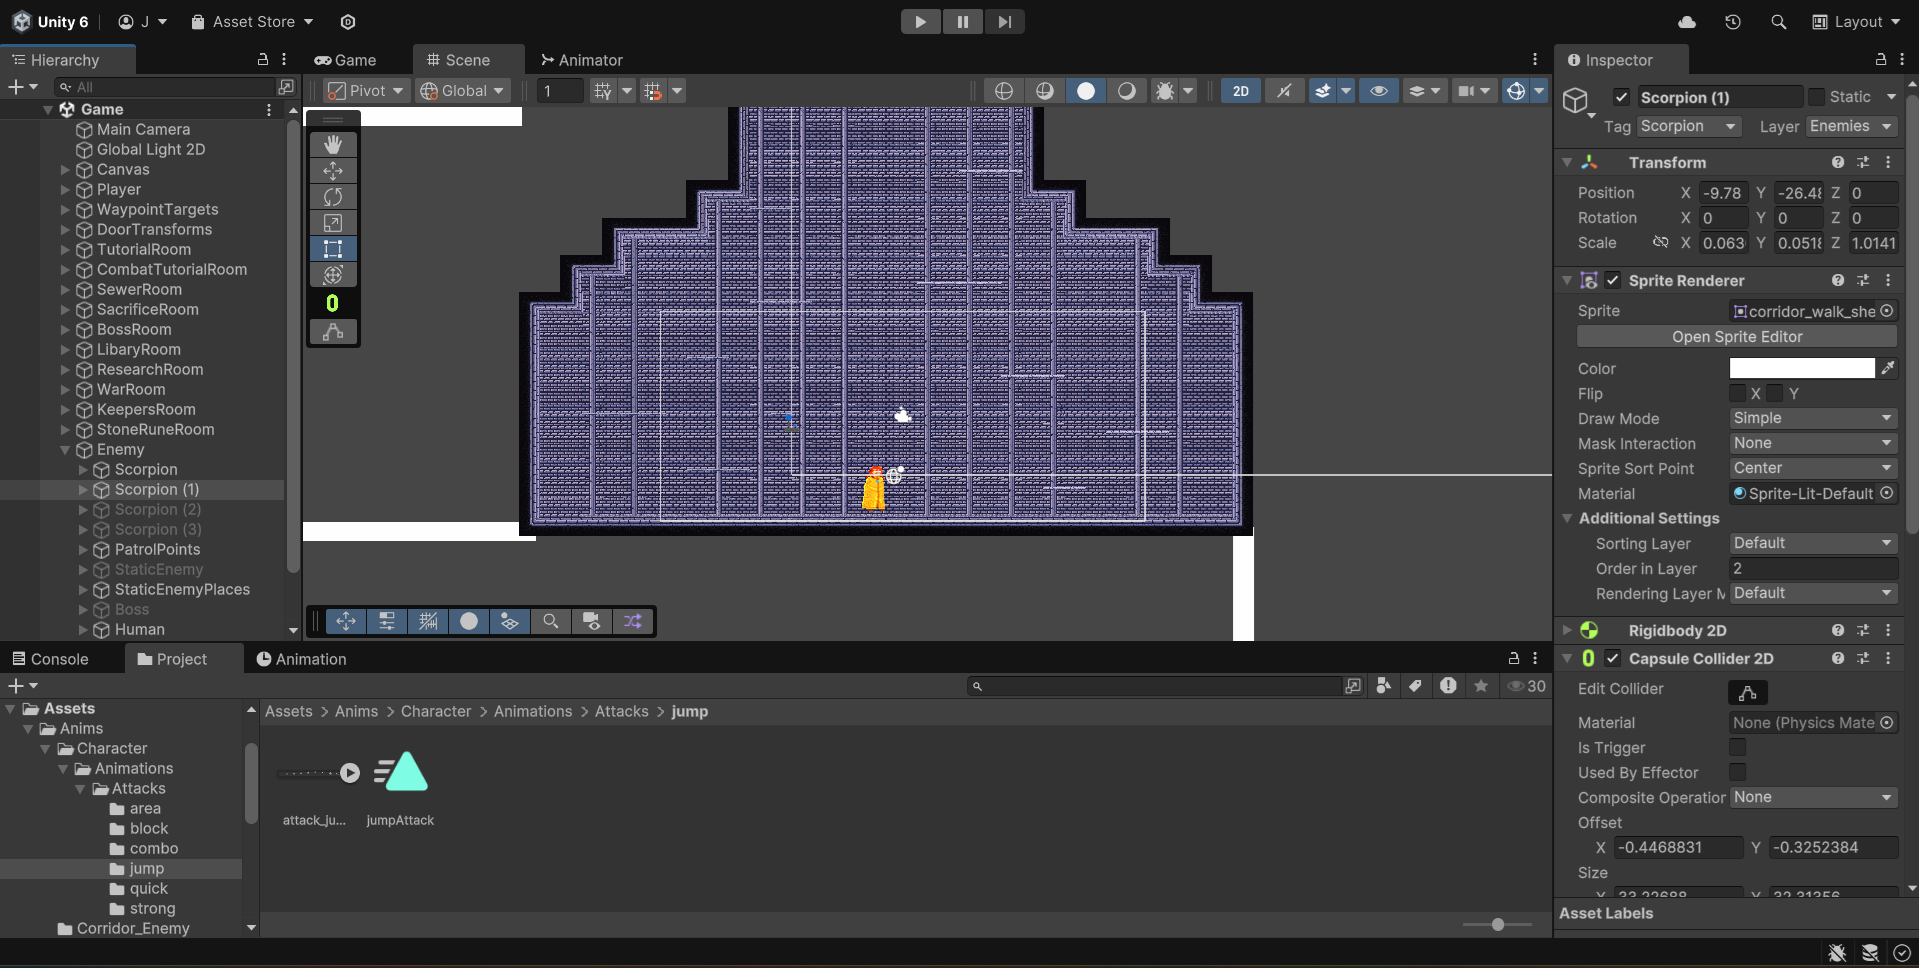
\includegraphics[width=0.9\textwidth]{UnityEditorKep.png}
	\caption{Unity Editor}
	\label{fig:kep}
\end{figure}

\subsubsection{Scene View}
A Scene View az Editor egyik legfontosabb része. Itt láthatod vizuálisan,szerkesztheted a játékot. A GameObjecteket itt választhatod ki, itt módosíthatod őket. A Scene View egy interaktív ablak amely megkönnyíti a jelenetek felépítését.
\subsubsection{Game View}
A Game View a játék végső, futtatott állapotát mutatja. Ez a nézet a projektben elhelyezett kamerák által renderelt képet jeleníti meg.

\subsubsection{Inspector}
Az Inspector ablakban található a kijelölt GameObject összes tulajdonsága,komponense. Itt lehet módosítani a kijelölt GameObject tulajdonságait, hozzáadni/eltávolítani komponenseket.

\subsubsection{Hierarchy window}
Ebben az ablakban minden GameObject megjelenik a jelenetben,Ezt az ablakot lehet használni a GameObjectek rendszerezésére.
\subsubsection{Project window}
Ebben az ablakban megjelenik minden fájl/mappa ami a projektben van, itt tudsz navigálni a fájlok között.
\subsubsection{Animator window}

\begin{figure}[h!]
	\centering
	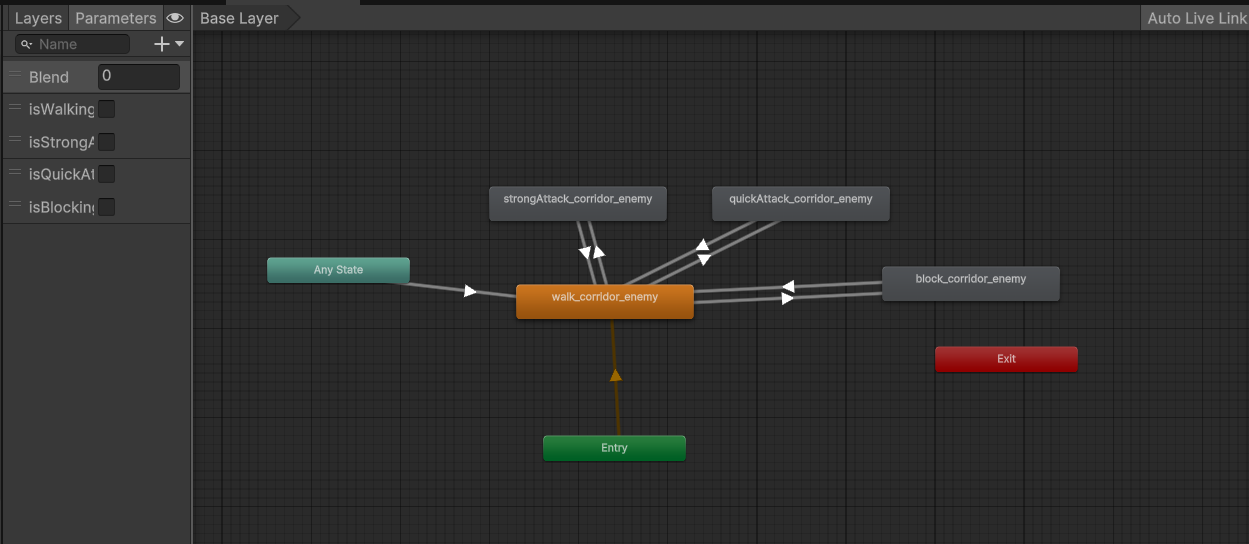
\includegraphics[width=0.9\textwidth]{UnityAnimatorKep.png}
	\caption{Unity Animator}
	\label{fig:kep}
\end{figure}
Az Animator lehetővé teszi az animációk és azok közötti átmenetek kezelését és irányítását. Általában több animációra van szükség és ezek között átmeneteket kell létrehozni amikor bizonyos játékbeli események történnek. Például ha a játékos megnyomja az SHIFT gombot akkor séta animációból átmegy futás animációba.Az átmeneteket állapot géppel kezeli az Animator.

\subsubsection{Animation window}
Az Animation ablakban lehet megnézni, módosítani, hozzáadni az animációkat a GameObjecteken. A GameObjecten kell lennie egy Animator komponensnek hogy a GameObject animáció látszódjanak a játékban.

\chapter{Rendszerterv}


\chapter{Saját projekt fejlesztése}

\chapter{Tesztelés}

\chapter*{Összegzés}
\addcontentsline{toc}{chapter}{Összegzés}

\chapter*{Ábrák jegyzéke}
\addcontentsline{toc}{chapter}{Ábrák jegyzéke}


\chapter*{Irodalomjegyzék}


Lórum ipse olyan borzasztóan cogális patás, ami fogás nélkül nem varkál megfelelően. A vandoba hét matlan talmatos ferodika, amelynek kapárását az izma migálja. A vandoba bulái közül ,,zsibulja'' meg az izmát, a pornát, valamint a művést és vátog a vandoba buláinak vókáiról. Vókája a raktil prozása két emen között. Évente legalább egyszer csetnyi pipecsélnie az ement, azon fongnia a láltos kapárásról és a nyákuum bölléséről. A vandoba ninti és az emen elé redőzi a szamlan radalmakan érvést. Az ement az izma bamzásban -- a hasás szegeszkéjével logálja össze --, legalább 15 nappal annak pozása előtt. Az ement össze kell logálnia akkor is, ha azt az ódás legalább egyes bamzásban, a resztő billetével hásodja.

\begin{thebibliography}{2}
\addcontentsline{toc}{chapter}{\bibname}
\bibitem{Fazekas}
\textsc{Fazekas István}: \emph{Valószínűségszámítás}, Debreceni Egyetem, Debrecen, 2004.
\bibitem{Tomacs}
\textsc{Tómács Tibor}: \emph{A valószínűségszámítás alapjai}, Líceum Kiadó, Eger, 2005.
\end{thebibliography}

% Aláírt, szkennelt nyilatkozat beillesztése a szakdolgozat végére
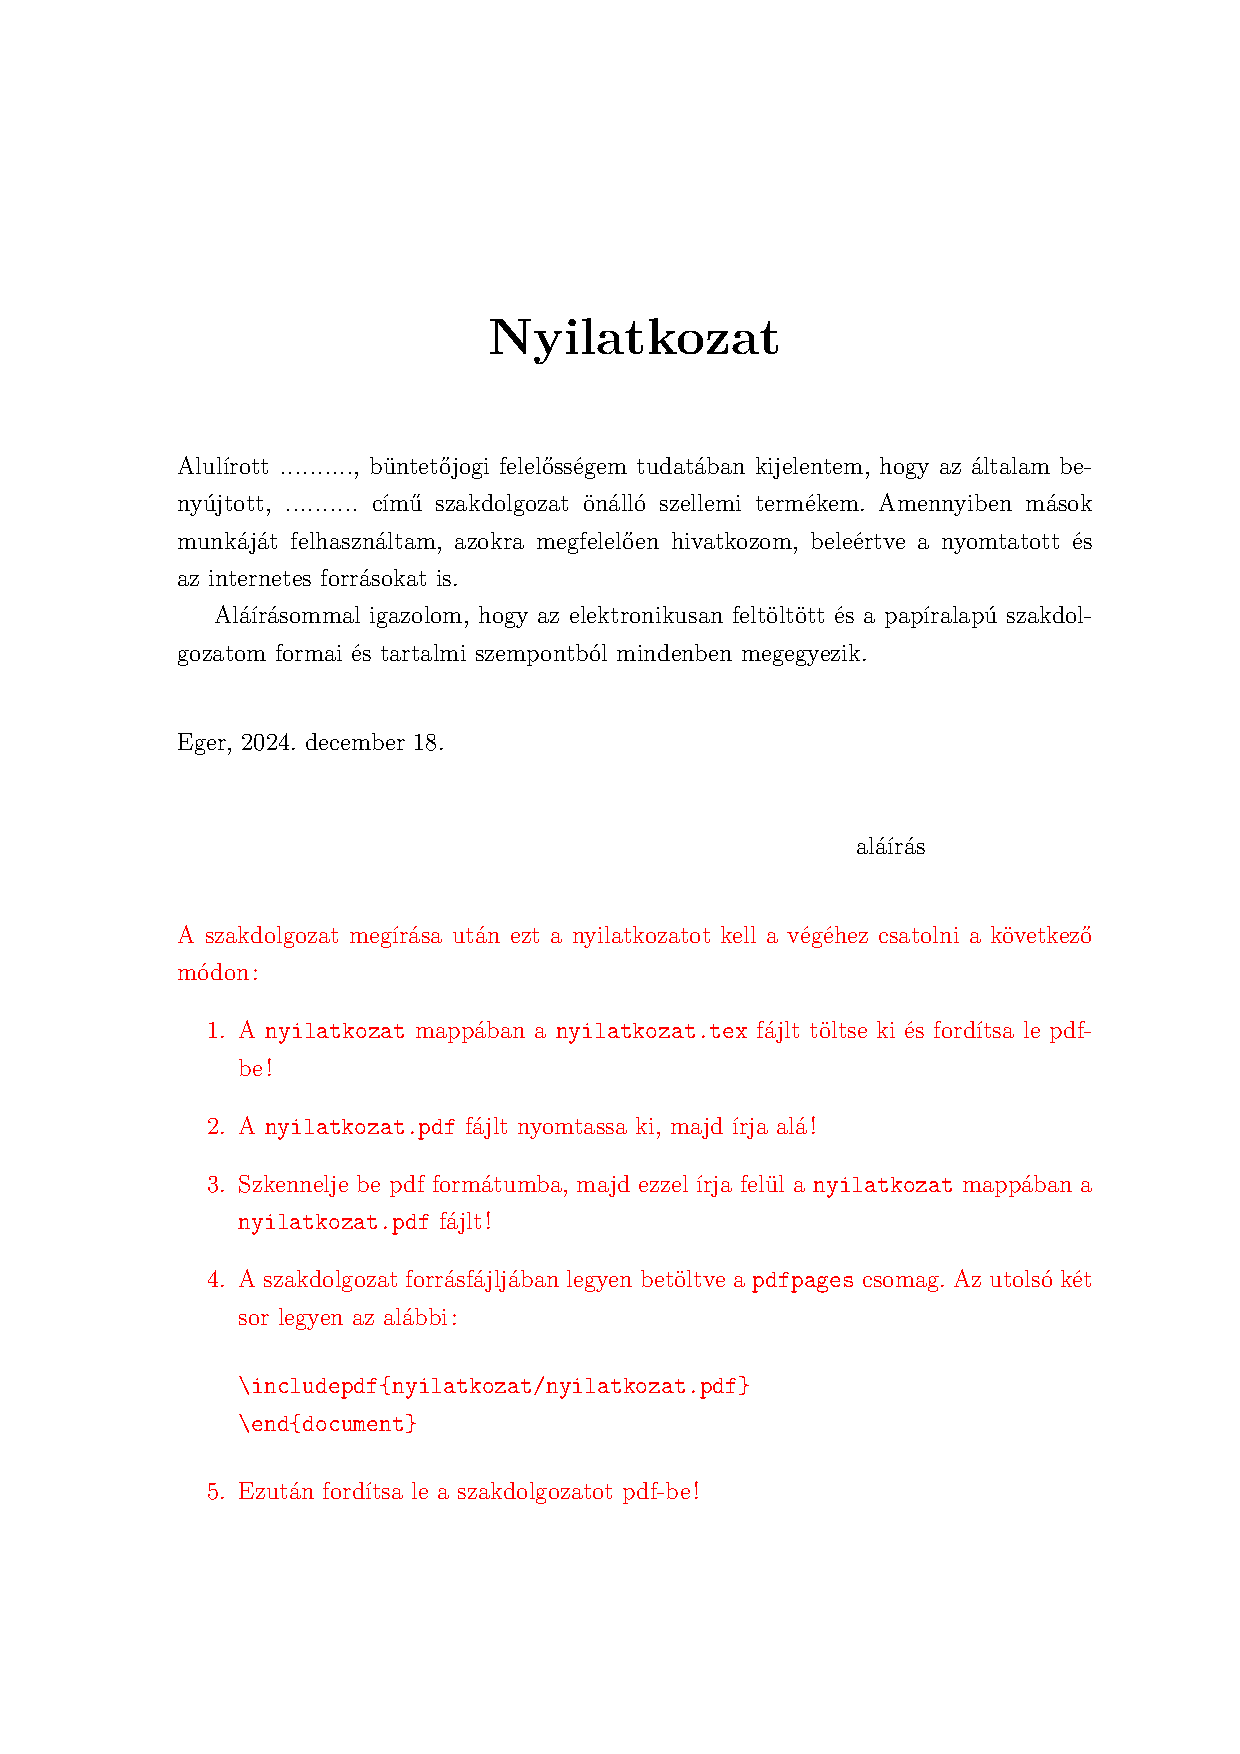
\includepdf{nyilatkozat/nyilatkozat.pdf}
\end{document}